\chapter{Triển khai hệ thống}

\section{Container hóa với Docker}

\subsection{Giới thiệu Docker}

Docker là một nền tảng mã nguồn mở được thiết kế để phát triển, đóng gói và chạy
các ứng dụng~\cite{docker}. Docker giải quyết bài toán ``chạy được trên máy tôi
nhưng không chạy được trên máy bạn'' bằng cách đóng gói ứng dụng cùng toàn bộ
phụ thuộc---thư viện runtime, biến môi trường, file cấu hình---vào một đơn vị
tiêu chuẩn gọi là \textit{container}. Đối với dự án này, Docker là thành phần
thiết yếu vì nó đảm bảo tính nhất quán tuyệt đối giữa môi trường phát triển cục
bộ, kiểm thử và sản xuất, đồng thời đơn giản hóa đáng kể quy trình triển khai
trên máy chủ.

\begin{figure}[h]
    \centering
    
\includegraphics[width=0.4\textwidth]{figures/docker_logo.png}
    \caption{Docker}
    \label{fig:docker_logo}
\end{figure}

\subsection{Cấu hình môi trường phát triển cục bộ}

Trong giai đoạn phát triển, Docker Compose được sử dụng để quản lý kiến trúc
đa container của hệ thống. File \texttt{docker-compose.yml} định nghĩa hai dịch
vụ hạ tầng cốt lõi:

\begin{itemize}
    \item \textbf{PostgreSQL 15:} Cơ sở dữ liệu quan hệ chính của hệ thống,
          được cấu hình với health check để đảm bảo sẵn sàng trước khi ứng dụng
          kết nối. Dữ liệu được lưu trữ bền vững qua Docker volume
          \texttt{postgres\_data}.

    \item \textbf{Kafka 4.0.0 (KRaft mode):} Message broker xử lý giao tiếp
          bất đồng bộ cho các luồng email và thông báo. Dự án sử dụng chế độ
          KRaft (không cần ZooKeeper), giảm đáng kể độ phức tạp vận hành.
          Dữ liệu Kafka được lưu trong volume \texttt{kafka\_data}.
\end{itemize}

Ứng dụng Spring Boot và giao diện React được chạy trực tiếp trên máy của nhà
phát triển (không trong container) để tận dụng tính năng hot-reload, giúp chu
kỳ phát triển nhanh hơn.

\begin{verbatim}
# Khởi động hạ tầng
docker compose up -d

# Chạy Backend
cd LMS_be && mvn spring-boot:run -pl library-bootstrap

# Chạy Frontend
cd LMS_fe && npm run dev
\end{verbatim}

\section{Dockerfile đa giai đoạn}

Để triển khai lên môi trường sản xuất, mỗi thành phần được đóng gói thành
Docker image riêng sử dụng kỹ thuật \textit{multi-stage build}---tách biệt
giai đoạn biên dịch và giai đoạn chạy nhằm tối thiểu hóa kích thước image
cuối cùng~\cite{docker_multistage}.

\subsection{Backend Dockerfile}

Dockerfile của Spring Boot bao gồm hai giai đoạn:

\begin{itemize}
    \item \textbf{Giai đoạn Build:} Sử dụng image \texttt{maven:3.9-eclipse-temurin-21-alpine}.
          Các file \texttt{pom.xml} được sao chép trước để Docker cache lớp
          phụ thuộc Maven---chỉ tải lại khi \texttt{pom.xml} thay đổi, không
          phải mỗi lần build. Sau đó toàn bộ mã nguồn được sao chép và build
          với lệnh \texttt{mvn package -DskipTests -pl library-bootstrap -am}.

    \item \textbf{Giai đoạn Runtime:} Sử dụng image \texttt{eclipse-temurin:21-jre-alpine}---
          chỉ chứa Java Runtime Environment, không có Maven hay mã nguồn.
          File JAR được sao chép từ giai đoạn build sang. Kích thước image
          cuối cùng giảm đáng kể so với image chứa đầy đủ JDK và Maven.
\end{itemize}

\subsection{Frontend Dockerfile}

Dockerfile của React cũng sử dụng hai giai đoạn:

\begin{itemize}
    \item \textbf{Giai đoạn Build:} Sử dụng \texttt{node:20-alpine}, cài đặt
          phụ thuộc qua \texttt{npm ci} và chạy \texttt{npm run build} (Vite)
          để tạo ra thư mục \texttt{/dist} chứa các file tĩnh đã được tối ưu.
          URL API được truyền vào lúc build qua build argument
          \texttt{VITE\_API\_BASE\_URL=/api/v1}.

    \item \textbf{Giai đoạn Runtime:} Sử dụng \texttt{nginx:alpine} phục vụ
          các file tĩnh từ \texttt{/usr/share/nginx/html}. Cấu hình Nginx
          của frontend được thiết lập để chuyển hướng tất cả các route về
          \texttt{index.html}, hỗ trợ React Router hoạt động đúng khi người
          dùng truy cập trực tiếp vào URL.
\end{itemize}

\section{Nginx --- Reverse Proxy}

\subsection{Vai trò của Nginx}

Nginx đóng vai trò là reverse proxy trung tâm, tiếp nhận toàn bộ traffic từ
bên ngoài trên cổng 80 và định tuyến đến đúng dịch vụ nội bộ~\cite{nginx}.
Kiến trúc này mang lại hai lợi ích chính: thứ nhất, các cổng nội bộ của từng
container (8080 cho Backend, 80 cho Frontend) không bị lộ ra internet; thứ hai,
client chỉ cần giao tiếp với một địa chỉ duy nhất.

\subsection{Cấu hình định tuyến}

File cấu hình \texttt{nginx/nginx.conf} định nghĩa ba quy tắc định tuyến:

\begin{itemize}
    \item \textbf{/ws} $\rightarrow$ Backend (WebSocket): Định tuyến các kết nối
          WebSocket STOMP/SockJS đến Spring Boot. Cần thiết lập
          \texttt{proxy\_http\_version 1.1} và header \texttt{Upgrade} để
          nâng cấp kết nối HTTP thành WebSocket. Thời gian chờ
          \texttt{proxy\_read\_timeout} được đặt là 3600 giây để duy trì
          kết nối real-time lâu dài.

    \item \textbf{/api/} $\rightarrow$ Backend (REST API): Tất cả các yêu cầu
          REST API được chuyển tiếp đến Spring Boot tại
          \texttt{http://spring-boot:8080}. Header \texttt{X-Real-IP} và
          \texttt{X-Forwarded-For} được thêm vào để Spring Boot ghi nhận
          địa chỉ IP thực của client.

    \item \textbf{/} $\rightarrow$ Frontend (React SPA): Toàn bộ các yêu cầu
          còn lại được chuyển đến container React. Frontend Nginx nội bộ
          xử lý việc phục vụ file tĩnh và hỗ trợ React Router.
\end{itemize}

\begin{figure}[h]
    \centering
    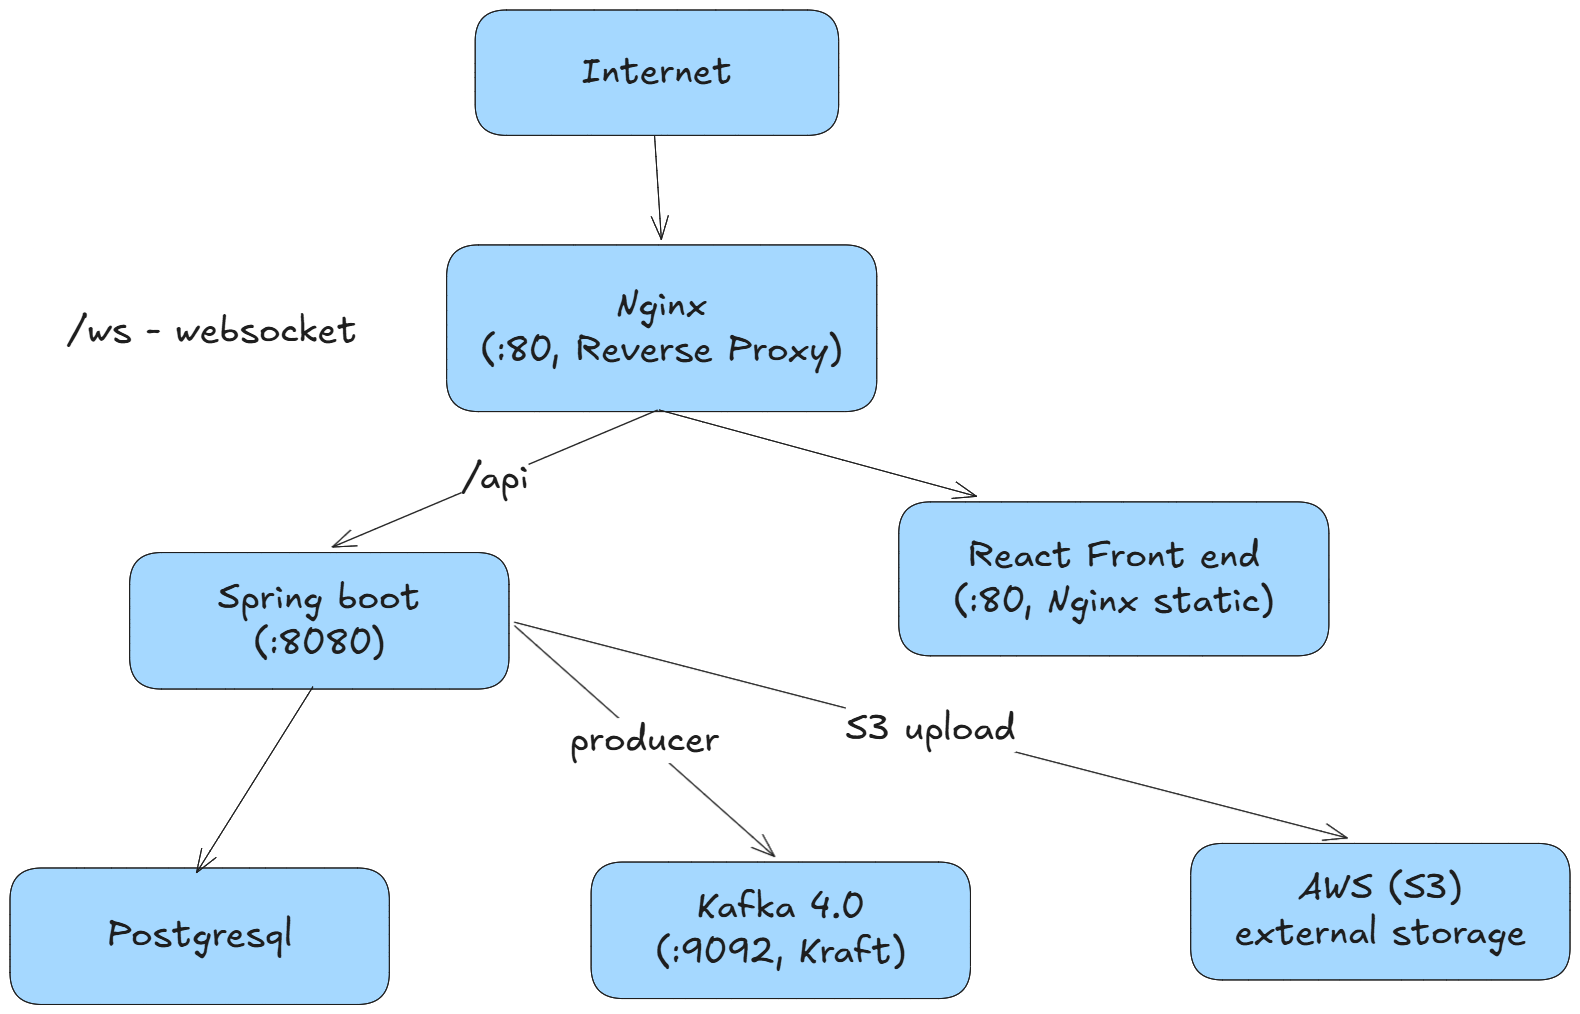
\includegraphics[width=0.85\textwidth]{figures/deployment_architecture.png}
    \caption{Kiến trúc triển khai hệ thống}
    \label{fig:deployment_arch}
\end{figure}

\section{Môi trường sản xuất}

\subsection{Docker Compose sản xuất}

File \texttt{docker-compose.prod.yml} mở rộng cấu hình phát triển bằng cách
thêm hai container mới---\texttt{spring-boot} và \texttt{frontend}---vào cùng
mạng Docker nội bộ với PostgreSQL, Kafka và Nginx. Tất cả năm dịch vụ giao tiếp
với nhau qua tên service (DNS nội bộ của Docker), không cần địa chỉ IP cố định.

Một điểm khác biệt quan trọng so với cấu hình phát triển là giá trị
\texttt{KAFKA\_CFG\_ADVERTISED\_LISTENERS} được thay đổi từ
\texttt{PLAINTEXT://localhost:9092} thành \texttt{PLAINTEXT://kafka:9092}.
Trong môi trường phát triển, Spring Boot chạy trên máy host nên dùng
\texttt{localhost}; trong môi trường container, Spring Boot nằm trong một
container khác và phải kết nối đến Kafka qua tên service Docker.

\begin{verbatim}
# Triển khai toàn bộ hệ thống
docker compose -f docker-compose.prod.yml up -d --build
\end{verbatim}

\subsection{Quản lý biến môi trường và bảo mật}

Tất cả thông tin nhạy cảm của hệ thống được quản lý thông qua file \texttt{.env}
và không bao giờ được đưa vào mã nguồn (được liệt kê trong \texttt{.gitignore}).
Bảng~\ref{tab:env_vars} liệt kê các nhóm biến môi trường chính.

\begin{table}[h]
\centering
\caption{Các nhóm biến môi trường của hệ thống}
\label{tab:env_vars}
\begin{tabular}{|l|p{5cm}|l|}
\hline
\textbf{Nhóm} & \textbf{Biến} & \textbf{Mục đích} \\
\hline
Cơ sở dữ liệu
  & \texttt{DATABASE\_URL} \newline
    \texttt{DATABASE\_USERNAME} \newline
    \texttt{DATABASE\_PASSWORD}
  & Kết nối PostgreSQL \\
\hline
JWT
  & \texttt{EXP\_TOKEN} \newline
    \texttt{EXP\_REFRESH\_TOKEN}
  & Thời hạn Access/Refresh token \\
\hline
OAuth2 Google
  & \texttt{GOOGLE\_CLIENT\_ID} \newline
    \texttt{GOOGLE\_CLIENT\_SECRET} \newline
    \texttt{OAUTH2\_REDIRECT\_URI}
  & Đăng nhập Google \\
\hline
Email
  & \texttt{MAIL\_SENDER\_USERNAME} \newline
    \texttt{MAIL\_SENDER\_PASSWORD}
  & Gửi email qua SMTP \\
\hline
AWS S3
  & \texttt{AWS\_ACCESS\_KEY} \newline
    \texttt{AWS\_SECRET\_KEY}
  & Lưu trữ file (ảnh bìa, tài liệu) \\
\hline
\end{tabular}
\end{table}

Khi triển khai lên máy chủ, file \texttt{.env} được sao chép trực tiếp lên
server và được tham chiếu qua chỉ thị \texttt{env\_file} trong Docker Compose.
Cách tiếp cận này đảm bảo không có thông tin đăng nhập nào được nhúng vào
Docker image hoặc lộ trong lịch sử git.

\subsection{Flyway Migration tự động}

Hệ thống sử dụng Flyway để quản lý phiên bản schema cơ sở dữ liệu. Khi
container Spring Boot khởi động, Flyway tự động thực thi các file migration
chưa được áp dụng theo thứ tự phiên bản trước khi ứng dụng nhận request.
Điều này đảm bảo schema cơ sở dữ liệu luôn đồng bộ với phiên bản ứng dụng
mà không cần can thiệp thủ công.

\begin{verbatim}
db/migration/
+-- V1__create_schema.sql   # Toan bo schema he thong
\-- V2__seed_data.sql       # Du lieu mau ban dau
\end{verbatim}

\subsection{Sơ đồ kiến trúc triển khai}

Hình~\ref{fig:deployment_detail} mô tả chi tiết luồng traffic từ người dùng
đến từng thành phần của hệ thống trong môi trường sản xuất.

\begin{figure}[h]
    \centering
    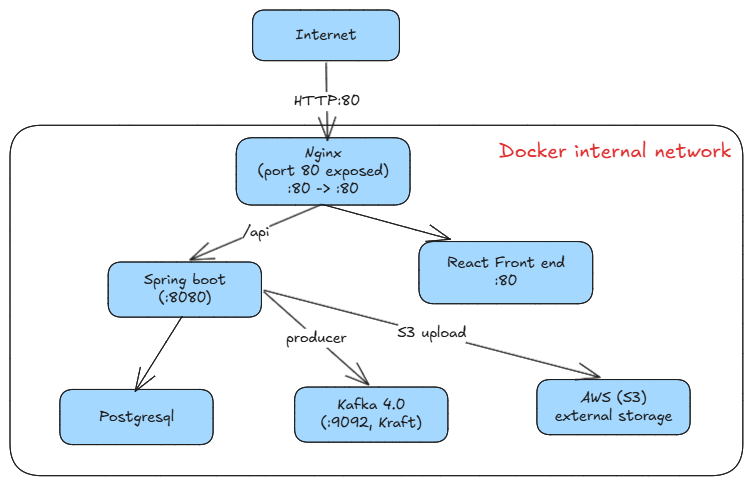
\includegraphics[width=\textwidth]{figures/deployment_detail.png}
    \caption{Luồng traffic qua các container trong môi trường sản xuất}
    \label{fig:deployment_detail}
\end{figure}

Toàn bộ năm container chạy trong cùng một Docker network nội bộ, giao tiếp
qua DNS tên service. Chỉ có Nginx container được ánh xạ cổng ra ngoài (cổng 80),
đảm bảo các dịch vụ nội bộ như PostgreSQL (5432) và Kafka (9092) không bị truy
cập trực tiếp từ internet.

\section{Quy trình triển khai}

Quy trình triển khai hệ thống lên một máy chủ Linux mới bao gồm các bước sau:

\begin{enumerate}
    \item \textbf{Chuẩn bị máy chủ:} Cài đặt Docker Engine và Docker Compose
          Plugin trên máy chủ Ubuntu.

    \begin{verbatim}
curl -fsSL https://get.docker.com | sh
    \end{verbatim}

    \item \textbf{Sao chép mã nguồn:} Clone repository về máy chủ.

    \begin{verbatim}
git clone <repository-url>
cd doan
    \end{verbatim}

    \item \textbf{Cấu hình môi trường:} Tạo file \texttt{.env} từ template và
          điền các giá trị thực tế (database credentials, API keys, v.v.).

    \begin{verbatim}
cp LMS_be/.env.example LMS_be/.env
# Chỉnh sửa LMS_be/.env với giá trị thực tế
    \end{verbatim}

    \item \textbf{Khởi động hệ thống:} Build image và khởi động tất cả container.

    \begin{verbatim}
docker compose -f docker-compose.prod.yml up -d --build
    \end{verbatim}

    \item \textbf{Kiểm tra trạng thái:} Xác nhận tất cả container đang chạy.

    \begin{verbatim}
docker compose -f docker-compose.prod.yml ps
docker compose -f docker-compose.prod.yml logs spring-boot
    \end{verbatim}
\end{enumerate}

Sau khi khởi động, Flyway tự động chạy các migration, sau đó hệ thống sẵn sàng
phục vụ tại địa chỉ \texttt{http://<server-ip>}.

\section{Hạ tầng mạng: VPS, Domain và HTTPS}

\subsection{Máy chủ ảo (VPS)}

Để một ứng dụng web có thể truy cập từ internet, hệ thống cần được triển khai
trên một máy chủ có địa chỉ IP công cộng hoạt động liên tục 24/7. Giải pháp
phổ biến nhất là thuê \textit{Virtual Private Server} (VPS)---một máy chủ ảo
được cấp phát tài nguyên CPU, RAM và ổ đĩa riêng biệt trên hạ tầng vật lý của
nhà cung cấp dịch vụ đám mây~\cite{vps}.

Đối với hệ thống thư viện này, cấu hình tối thiểu được đề xuất là \textbf{2GB
RAM} do Kafka yêu cầu khoảng 512MB bộ nhớ để hoạt động ổn định cùng với Spring
Boot và PostgreSQL. Bảng~\ref{tab:vps_options} so sánh một số nhà cung cấp VPS
phổ biến.

\begin{table}[h]
\centering
\caption{So sánh các nhà cung cấp VPS phổ biến}
\label{tab:vps_options}
\begin{tabular}{|l|c|c|c|}
\hline
\textbf{Nhà cung cấp} & \textbf{RAM} & \textbf{Giá} & \textbf{Ghi chú} \\
\hline
Hetzner Cloud (CX22)   & 4 GB & €4/tháng  & Giá rẻ, datacenter EU \\
\hline
DigitalOcean (Basic)   & 1 GB & \$6/tháng & Phổ biến, dễ sử dụng \\
\hline
Vultr (Regular)        & 1 GB & \$5/tháng & Nhiều khu vực \\
\hline
Oracle Cloud Free Tier & 1 GB & Miễn phí  & Vĩnh viễn, ARM architecture \\
\hline
\end{tabular}
\end{table}

\subsection{Tên miền (Domain)}

Sau khi có VPS với địa chỉ IP công cộng (ví dụ: \texttt{103.45.67.89}), hệ
thống đã có thể truy cập trực tiếp qua IP. Tuy nhiên, để có địa chỉ thân
thiện và dễ nhớ, cần mua thêm một \textit{tên miền}---ví dụ
\texttt{smartlibrary.vn} hoặc \texttt{lms-hcmut.com}. Tên miền được đăng ký
thông qua các nhà cung cấp như GoDaddy, Namecheap hoặc các nhà đăng ký tên
miền Việt Nam.

Sau khi mua tên miền, cần cấu hình bản ghi DNS loại \textbf{A record} trỏ tên
miền về địa chỉ IP của VPS. Quá trình phân giải DNS diễn ra tự động, thông
thường có hiệu lực trong vòng vài phút đến 24 giờ. Hình~\ref{fig:dns_flow}
minh họa luồng kết nối từ người dùng đến hệ thống.

\begin{figure}[h]
    \centering
    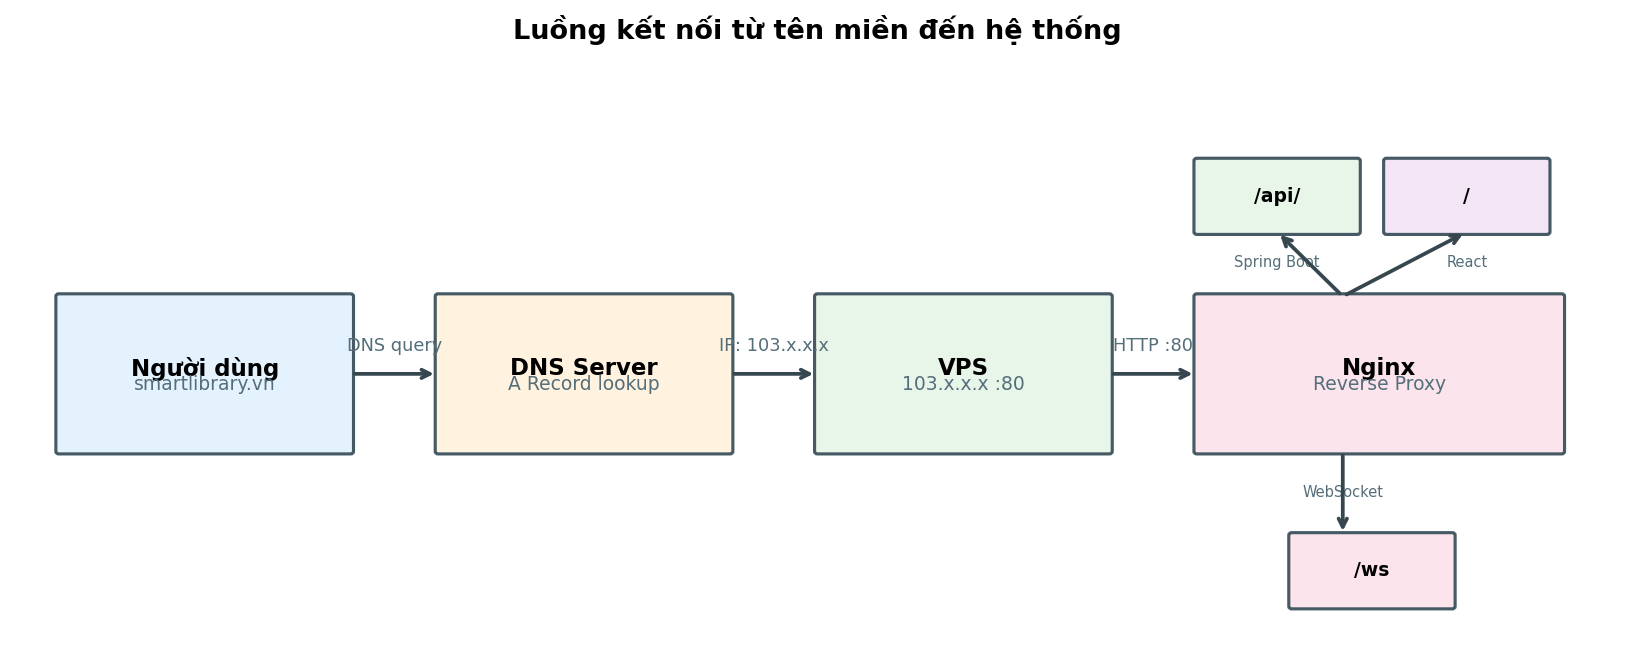
\includegraphics[width=0.85\textwidth]{figures/dns_flow.png}
    \caption{Luồng kết nối từ tên miền đến hệ thống}
    \label{fig:dns_flow}
\end{figure}

\subsection{HTTPS và SSL/TLS Certificate}

Các trình duyệt hiện đại cảnh báo người dùng khi truy cập trang web qua HTTP
không mã hóa. Để bảo mật dữ liệu truyền tải---đặc biệt là JWT token, thông
tin đăng nhập và dữ liệu cá nhân---hệ thống cần được cấu hình HTTPS thông qua
SSL/TLS certificate~\cite{letsencrypt}.

\textbf{Let's Encrypt} là tổ chức phi lợi nhuận cung cấp SSL certificate hoàn
toàn miễn phí và tự động. Công cụ \textbf{Certbot} tích hợp trực tiếp với
Nginx, tự động xác minh quyền sở hữu tên miền, cấp certificate và cập nhật
cấu hình Nginx để lắng nghe trên cổng 443 (HTTPS):

\begin{verbatim}
# Cài đặt Certbot
apt install certbot python3-certbot-nginx

# Cấp certificate và tự động cấu hình Nginx
certbot --nginx -d smartlibrary.vn -d www.smartlibrary.vn
\end{verbatim}

Certificate Let's Encrypt có hiệu lực 90 ngày và được Certbot tự động gia hạn
qua cron job, không cần can thiệp thủ công.

\subsection{Tổng chi phí vận hành}

Bảng~\ref{tab:hosting_cost} tổng hợp chi phí ước tính để vận hành hệ thống
trong môi trường sản xuất với tên miền và HTTPS đầy đủ.

\begin{table}[h]
\centering
\caption{Chi phí vận hành hệ thống ước tính}
\label{tab:hosting_cost}
\begin{tabular}{|l|c|c|l|}
\hline
\textbf{Thành phần} & \textbf{Chi phí} & \textbf{Chu kỳ} & \textbf{Ghi chú} \\
\hline
VPS (Hetzner CX22)   & ~90.000đ  & Tháng   & 4GB RAM, 2 vCPU \\
\hline
Tên miền \texttt{.com} & ~300.000đ & Năm     & Qua Namecheap, GoDaddy \\
\hline
SSL Certificate      & Miễn phí  & 90 ngày & Let's Encrypt, tự gia hạn \\
\hline
AWS S3 (lưu trữ)     & ~23.000đ  & Tháng   & 1GB storage + transfer \\
\hline
\textbf{Tổng}        & \textbf{$\approx$140.000đ} & \textbf{Tháng} & Chưa tính domain năm đầu \\
\hline
\end{tabular}
\end{table}

\noindent Chi phí vận hành thấp này cho thấy hệ thống hoàn toàn khả thi để
triển khai thực tế trong môi trường trường đại học với ngân sách hạn chế.
